\label{cha:grundlagen}
Als Fundament für die weitere Arbeit sollen zunächst einige Grundlagen thematisiert werden. Um das Vorhaben und das Vorgehen dieser Arbeit besser nachvollziehen zu können, wird zunächst das Modell der \textit{Tetrade der Medieneffekte} vorgestellt. Hierbei handelt es sich um eine Idee von Marshall McLuhan, welcher sich mit den Effekten beschäftigt, die ein Medium mit sich bringt. Er hat festgestellt, dass im Wesentlichen vier Effekte von Interesse sind, welche er mit den folgenden Fragen bestimmen will \citep{mcluhan1977laws}:

\begin{enumerate}
\item What does the medium enhance?
\item What does the medium make obsolete?
\item What does the medium retrieve that had been obsolesced earlier?
\item What does the medium reverse or flip into when pushed to extremes?
\end{enumerate}

So stellt \cite{mcluhan1977laws} fest, dass das Radio eine unmittelbare und auditive Art der Kommunikation beförderte. Im gleichen Moment wurde dadurch die Bedeutsamkeit von Printmedien geschwächt. Hierdurch hat die vorangegangene auditive Kommunikation, welche durch die Einführung von Printmedien obsolet wurde, wieder an Bedeutung gewonnen. Wenn man nun das Medium an sein Limit bringt, dann befördert dies die Entwicklung hin zum Fernsehen \citep{mcluhan1977laws}.

Analog hierzu soll das Ziel der Einführung des Hyperaudio"=Plugins sein, Medien wie Podcasts und Hörbücher zu erweitern, um Kurseinheiten und Präsenzveranstaltungen überflüssig zu machen. Hierdurch würde das Bildungsradio wieder reaktiviert. Wenn Hyperaudio an seine Grenzen gebracht wird, würde dies zu Video beziehungsweise Hypervideo führen. Mit diesen Gedanken im Hinterkopf werden nun die Grundlagen für diese Arbeit vorgestellt. Die betrachteten Themen beschäftigen sich ebenfalls mit Medien und deren Effekten.

\section{Moodle}
\label{sec:moodle}
Bei Moodle (Modular Object-Oriented Dynamic Learning Environment) handelt es sich um ein frei verfügbares Open-Source-Learningmanagementsystem (GNU Public License), mit dem Internet-basierte Kurse entwickelt und durchgeführt werden können \citep{moodle2015was}. Ziel der Lernplattform ist es, den Lehrenden, Administratoren und Lernenden ein robustes, sicheres und integriertes System zu liefern, mit dessen Hilfe sie eine personalisierte Lernumgebung gestalten können \citep{moodle2018about}. Unter dieser Zielsetzung ist Moodle als Lernplattform weltweit verbreitet und hat aktuell\footnote{Stand: 28.07.2018} 101.447 registrierte Seiten in 232 Ländern mit insgesamt mehr als 130 Millionen Benutzern \citep{moodle2018stats}.

Zugriff auf Moodle erhält der Nutzer über die Startseite, welche auf die eigenen Bedürfnisse angepasst werden kann. Die Grundstruktur von Moodle ist, wie in Abbildung \ref{fig:MoodleAufbau} zu sehen, anhand von Kursbereichen und Kursen organisiert. Kurse werden wiederum als Seiten repräsentiert, auf welchen die Lehrenden Arbeitsmaterialien und Aktivitäten für die Studierenden bereitstellen können. Kurse werden üblicherweise in einzelne Kursabschnitte unterteilt, in welchen die Arbeitsmaterialien und Aktivitäten eingebunden werden. Kursseiten können durch Blöcke noch um weitere zusätzliche Informationen angereichert werden.

Ein Beispiel für eine Kursseite ist in Abbildung \ref{fig:MoodleKursseitenbeispiel} anhand des Kurses \glqq Einführung in Mensch-Computer-Interaktion\grqq{} zu sehen. Auf der linken Seite sind innerhalb der Navigation die einzelnen Kursabschnitte, hier als Kurseinheiten beziehungsweise Einführung  benannt, sichtbar. Unterhalb der Navigation sowie auf der rechten Seite sind die verschiedenen Blöcke (z.B. \glqq Aktivitäten\grqq{}, \glqq Suche in Foren\grqq{} oder \glqq Neue Ankündigungen\grqq{}) innerhalb des Kurses angeordnet. Im mittleren Bereich befinden sich untereinander die Beschreibungen der einzelnen Kursabschnitte mit Links zu den verwendeten Arbeitsmaterialien und Aktivitäten.

Die vorab beschriebenen Kurse werden wiederum innerhalb von Kursbereichen organisiert. Es ist auch ein mehrstufiges Kursbereichssystem umsetzbar \citep{moodle2015aufbau}.

\begin{figure}[h!]
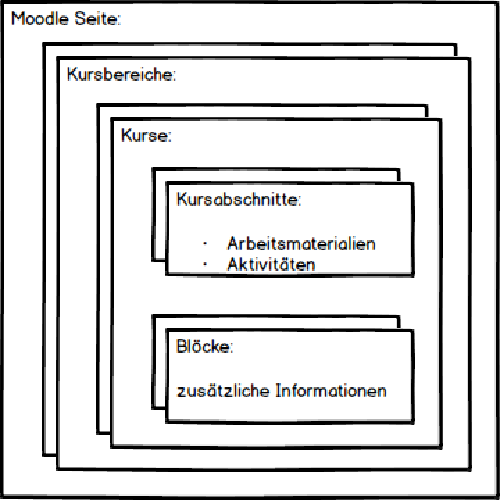
\includegraphics[width=.5\textwidth,center]{MoodleAufbau.pdf}
\caption{\label{fig:MoodleAufbau}Schematischer Aufbau einer Moodle Seite}
\end{figure}

\begin{figure}[h!]
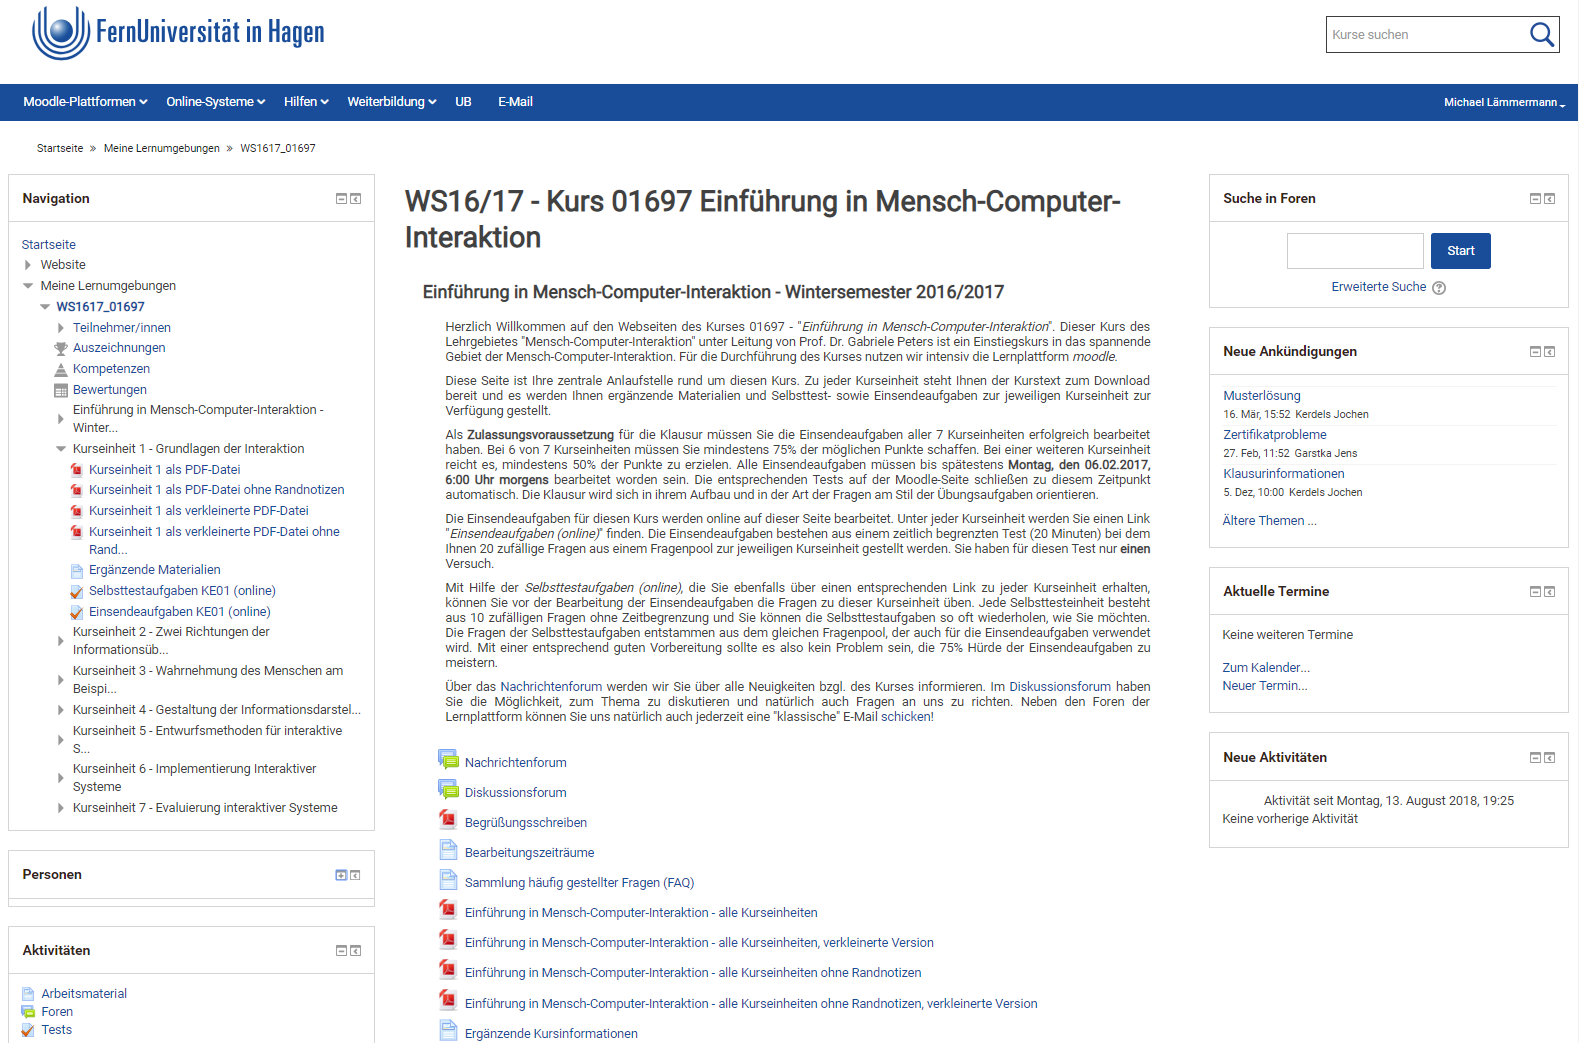
\includegraphics[width=\textwidth,center]{MoodleKursseitenbeispiel.png}
\caption{\label{fig:MoodleKursseitenbeispiel}Kursseite des Kurses \glqq Einführung in Mensch-Computer-Interaktion\grqq{} \citep{fernuniversitaet2018mensch}}
\end{figure}

%behauptung?
Technisch baut Moodle auf einem Aufbau aus Webserver und Datenbank unter Verwendung von PHP (PHP: Hypertext Preprocessor) auf. Um die zum Ziel gesetzte Personalisierbarkeit zu erreichen, setzt Moodle unter anderem auf ein Plugin-System. Plugins werden in über 50 verschiedene Plugin-Typen kategorisiert, wobei jeder dieser Typen dazu dient, einen speziellen Bereich von Moodle zu erweitern beziehungsweise anzupassen \citep{moodle2017plugin}.


%%%%%%%%%%
\section{Kooperation im Lernumfeld}
\label{sec:kooperativeslernen}
\glqq Lernen ist in vieler Hinsicht ein sozialer Prozess, der kulturelle Einflüsse einschließt sowie soziale Aktivitäten und gemeinsames Problemlösen umfasst\grqq{} \citep{reinmann1995kooperation}. %Diese Aussage macht die Bedeutung von Kooperation im Lernumfeld klar. 
%\textbf{Anhand dieser Aussage lässt sich schon grob erkennen, was unter Kooperation im Lernumfeld zu verstehen ist und welche Bedeutung dieser zugeordnet wird.}
Weitgefasst versteht man unter kooperativem Lernen eine Situation, in der zwei oder mehrere Personen zusammen lernen oder versuchen, zusammen zu lernen \citep{dillenbourg1999collaborative}.
%\todo[inline]{Verknüpfung}

Während in dieser Arbeit, wie im deutschsprachigen Raum üblich, keine Unterscheidung zwischen dem \textit{kooperativen} und dem \textit{kollaborativen} Lernen vorgenommen wird, werden die Begriffe außerhalb des deutschsprachigen Raums häufig differenziert betrachtet \citep{reinmann2002analyse}. Eine differenzierte Betrachtung der beiden Begriffe liefert \cite{dillenbourg1995evolution}. Demnach handelt es sich um \textit{Kooperation}, wenn eine Problemlösung durch die Arbeitsteilung unter den Mitgliedern einer Gruppe erreicht wird, wobei jedes Mitglied für einen Teil der Problemlösung verantwortlich ist.
Bei \textit{Kollaboration} wird die Problemlösung hingegen durch gemeinsames Engagement der Gruppenmitglieder bei koordiniertem Vorgehen zur Problemlösung erreicht.
Als Beispiel kann eine Gruppenarbeit mit der Aufgabe, mehrere Textabschnitte zusammenzufassen, betrachtet werden.
Bei einem kooperativen Vorgehen wäre zunächst jeweils ein Gruppenmitglied für die Zusammenfassung genau eines Textabschnittes verantwortlich. In einem zweiten Schritt würden dann die einzelnen Teilergebnisse zu einem Ergebnis zusammengefasst. Bei einem kollaborativen Vorgehen wiederum würden alle Gruppenmitglieder die einzelnen Textabschnitte gemeinsam zusammenfassen.

Dem kooperativen Lernen werden positive Effekte zugesprochen, unter anderem bezüglich der Lernmotivation \citep{reinmann1995kooperation,dillenbourg1999collaborative}. So wird beispielsweise beim Lernen durch Lehren, einer speziellen Form des kooperativen Lernens, die Motivation der Beteiligten erhöht. Gleichzeitig werden sowohl beim Lehrenden als auch beim Lernenden effektive Lernprozesse in Gang gesetzt \citep{reinmann1995kooperation}.

\cite{reinmann2002analyse} beschreiben auch, welche Probleme bei netzbasierten Umgebungen entstehen können. So können neben technischen Problemen auch Widerstände seitens der Nutzer vorliegen. Oftmals ist es schwer, die Gruppenmitglieder dazu zu bringen, aktiv an den netzbasierten Szenarien teilzunehmen. Auch besteht das Problem, dass in netzbasierten Umgebungen weniger individuelles als kollektives Wissen geteilt wird als in Face-to-Face-Situationen. Aufgrund der fehlenden sozialen Hinweisreize und der Anonymität kann \glqq es leicht zu unkontrollierter Kommunikation und heftigen Gefühlsausbrüchen, dem sog. Flaming, kommen\grqq{} \citep{reinmann2002analyse}.


%%%%%%%%%%
\section{Hypermedia}
Bevor mit der genauen Konzeption und Implementierung des Hyperaudio"=Plugins begonnen werden kann, werden \textit{Hypermedia} im Allgemeinen betrachtet. Dabei soll zunächst eine Begriffsklärung durchgeführt werden. Aus diversen Erfahrungen mit \textit{Hypermedia} können Rückschlüsse für das zu entwickelnde Moodle-Plugin und die zugrundeliegende Interpretation von \textit{Hyperaudio} gezogen werden.


%%%%%%%%%%
\subsection{Grundbegriffe}
Zu Beginn wird zunächst der Begriff \textit{Multimedia} betrachtet. Unter \textit{Multimedia} wird die Bereitstellung von Informationen mittels verschiedener Formate, beispielsweise Text, Audio, Bilder oder Video, bezeichnet \citep{mayer2009multimedia,moos2010multimedia}.

Der Begriff \textit{Hypermedia} wurde das erste Mal von Ted Nelson 1965 verwendet \citep{nelson1965complex}. In seinem Paper beschreibt er detailliert, was er sich unter einem \textit{Hypertext} vorstellt. Hierunter versteht er ein Dokument bestehend aus geschriebenen oder bildhaften Inhalten, welche in solch einer komplexen Art und Weise miteinander verbunden sind, dass sie nicht mehr auf Papier dargestellt werden können. Es kann Zusammenfassungen, Karten über die Inhalte und deren Zusammenhänge, Annotationen, Ergänzungen oder Anmerkungen von Wissenschaftlern, die das Dokument begutachtet haben, enthalten. Nelson beschreibt das Kriterium für den Präfix \textit{hyper} damit, dass diese Objekte nicht durch eine Konvertierung in ein einfaches lineares Medium, wie beispielsweise eine Zeichenkette umgewandelt werden können. Der wesentliche Punkt ist also, dass es sich beim Arbeiten mit \textit{Hypermedia} um ein nicht-lineares Vorgehen handelt.

Genauer betrachtet stellt das, was \cite{nelson1965complex} sich als \textit{Hypertext} vorgestellt hatte, nach \cite{nielsen2013multimedia} bereits eine Form von \textit{Hypermedia} dar. Auch wenn die beiden Begriffe \textit{Hypertext} und \textit{Hypermedia} synonym verwendet werden können, werden bei strikter Betrachtung bei \textit{Hypertext} ausschließlich Texte miteinander verbunden, während bei \textit{Hypermedia} auch andere Medien eingebunden werden können. Gemeinsam haben beide Arten jedoch, dass der Betrachter keinen linearen Weg vorgegeben hat, sondern von einem Knoten zum anderen springen kann und sich somit seinen Weg selbst aussucht. Demnach stellt \textit{Hypermedia} eine nicht-lineare Variante von \textit{Multimedia} dar.

Nach dieser Logik handelt es sich bei \textit{Hyperaudio} in seiner klassischen Form eigentlich um reine Audiosequenzen, die miteinander verknüpft sind, wobei der Zuhörer selbst entschieden kann, in welcher Reihenfolge er diese abspielt \citep{zumbach2006learning}.


%%%%%%%%%%
\subsection{Lernen mit Hypermedia}
\label{sub:LernenMitHypermedia}
Wissenschaftler beschäftigen sich schon seit vielen Jahren damit, festzustellen, welche Effekte der Einsatz von \textit{Multimedia}, \textit{Hypertext} und \textit{Hypermedia} auf den Lernerfolg von Lernenden hat.

%In der Arbeit von \cite{moos2010multimedia} wird eine Analyse von etlichen Arbeiten zu diesem Thema durchgeführt. \cite{moos2010multimedia} konzentrieren sich hierbei vor allem auf den Einfluss auf die Motivation der Lernenden. Dennoch wird auch auf andere Aspekte der drei verschiedenen E-Learning Methoden \textit{Multimedia}, \textit{Hypertext} und  \textit{Hypermedia} im Vergleich zu klassischen Lehrmethoden eingegangen.

\cite{mayer2009multimedia} konnte im Laufe seiner Untersuchungen positive Effekte beim Einsatz von \textit{Multimedia} nachweisen. So schnitten Studenten bei einem Transfertest besser ab, wenn sie mit Text und Bildern lernten, als wenn sie ausschließlich mit Text lernten. \cite{mayer2009multimedia} knüpft dieses Ergebnis aber an folgende Prinzipien, welche beim Einsatz von \textit{Multimedia} befolgt werden müssen:

\begin{itemize}
 \item  Kohärenz: irrelevante Wörter, Töne und Bilder sollten vermieden werden
 \item	Signalisieren: essentielle Inhalte sollten hervorgehoben sein
 \item	Redundanz: Text sollte ausschließlich auditiv statt auditiv und visuell in Multimediapräsentationen wiedergegeben werden
 \item	Räumliche Nähe: zusammengehörige Texte und Bilder sollten nah beieinander statt weit entfernt auf der Seite beziehungsweise dem Bildschirm dargestellt werden
 \item	Zeitliche Nähe: zusammengehörige Texte und Bilder sollten gleichzeitig statt nacheinander auf der Seite beziehungsweise dem Bildschirm dargestellt werden
 \item	Segmentierung: temporeiche, komplexe Multimedia–Lektionen sollten in benutzerfreundlichen Portionen statt im Ganzen präsentiert werden
 \item	Vorbereitung: der Lernende sollte die Begrifflichkeiten und Merkmale der Lektion kennen
 \item	Modalität: Text sollte auditiv statt visuell wiedergegeben werden
 \item	Personalisierung: Texte sollten in dialogorientiertem Stil statt in formellem Stil wiedergegeben werden
 \item	Stimme: Text sollte von einer freundlichen menschlichen Stimme statt einer Computerstimme wiedergegeben werden
\end{itemize}

Im Gegenzug verweisen \cite{moos2010multimedia} auf Arbeiten, nach denen eine Herausforderung bei \textit{Multimedia} und somit auch bei \textit{Hypermedia} darin besteht, dass die kognitive Aufnahmekapazität der Studierenden überschritten werden kann, wenn Informationen sowohl aus einem Text als auch aus einem Diagramm entnommen werden sollen (Mayer und Moreno; van Merrienboer und Ayres, nach \cite{moos2010multimedia}). Dies beruht auf der Annahme der Cognitive Load Theory, welche dem Arbeitsgedächtnis nur eine begrenzte Kapazität zuspricht (Sweller; van Merrienboer und Sweller, nach \cite{moos2010multimedia}). Diesem Problem ist laut \cite{mayer2009multimedia} mit den oben genannten Prinzipien zu begegnen, da diese darauf abzielen, die begrenzte Kapazität besser zu nutzen.

Ebenso wie \textit{Multimedia} bietet \textit{Hypertext} Vorteile. Diese bestehen beispielsweise darin, dass der Studierende den Lernweg bestimmen kann, der am besten auf seine Bedürfnisse angepasst ist. Auf der anderen Seite ist hierzu aber eine ausreichende Vorkenntnis im entsprechenden Lernbereich notwendig, um die Entscheidung treffen zu können, wie dieser Weg aussehen soll. Des Weiteren wirkt sich auch ein fehlendes Interesse des Studierenden negativ auf die Effektivität der \textit{Hypertext}-Lernumgebung aus (Lawless und Kulikowich, nach \cite{moos2010multimedia}).

Es ist nun also nicht verwunderlich, dass \textit{Hypermedia} als Verschmelzung von \textit{Multimedia} und \textit{Hypertext} ebenfalls einige Herausforderungen mit sich bringt \citep{moos2010multimedia}. Scott und Schwartz (nach \cite{moos2010multimedia}) fordern für das Lernen mit \textit{Hypermedia} eine Balance zwischen effektiver Navigation und Inhaltsverständnis. Dies soll durch Prozesse zur Überwachung des eigenen Lernfortschritts erreicht werden, wohingegen Untersuchungen ergeben haben, dass viele Studierende Schwierigkeiten dabei haben, diese Prozesse korrekt anzuwenden \citep{moos2010multimedia}.


\subsection{Hyperaudio-Repräsentation von Kurseinheiten}
\label{sec:hyperaudio}
\label{sec:audiocues}
\textit{Hyperaudio} als Sonderform von \textit{Hypermedia} bringt spezielle Probleme mit sich. So weisen \cite{donker2007gestaltung} auf die Herausforderungen bei der Gestlatung von \textit{Hyperaudio}-Anwendungen hin, welche unter anderem darin bestehen, dem Hörer die Hyperlinks innerhalb einer \textit{Hyperaudio}-Anwendung sinnvoll darzustellen. Bei ihrer Untersuchung kamen \cite{donker2007gestaltung} zu dem Ergebnis, \glqq dass sowohl eine Verdeutlichung von Links durch das Voranstellen eines Tons als auch die Variante durch das
Ändern des Alters des Sprechers zu guten Ergebnissen hinsichtlich des Erkennens des Links
führen.\grqq{} Die genannten vorangestellten Töne werden auch als \textit{Audio Cues} bezeichnet.

Bei einer auditiven Repräsentation von Kurseinheiten stellen sich einige Herausforderungen, denen ebenfalls mit den Erkenntnissen von \cite{donker2007gestaltung} begegnet werden kann:

\begin{itemize}
\item Wie können spezielle Textpassagen (Auflistungen, Beispiele, Aufgaben, Definitionen, Algorithmen etc.) nachvollziehbar wiedergegeben werden?
\item Wie können Zitate kenntlich gemacht werden?
\item Wie soll mit Ausdrücken in Klammern umgegangen werden?
\item Wie soll der Hörer auf Fußnoten hingewiesen werden?
\item Wie sollen Marginalien bei der Vertonung berücksichtigt werden?
\item Wie kann der Hörer über Querverweise informiert werden?
\end{itemize} 

In Anlehnung an \cite{donker2007gestaltung} könnte mit dem Einsatz verschiedener Audio Cues und Sprecher gearbeitet werden. Auch wäre ein Einsatz von \textit{Resonance Audio}\footnote{https://developers.google.com/resonance-audio/} von \textit{Google} denkbar. Damit wäre es möglich, durch unterschiedliche Positionierung im Raum oder durch Verwendung verschiedener Audio-Kanäle den gerade gesprochenen Inhalt zu kategorisieren. Zusätzlich sollten auch bei der Vertonung von Kurseinheiten die Prinzipien von \cite{mayer2009multimedia} (vgl. Abschnitt \ref{sub:LernenMitHypermedia}) beachtet werden.

Unter Berücksichtigung der soeben genannten Herausforderungen und Lösungsideen müssen für eine auditive Repräsentation der Kurseinheiten deren Inhalte entsprechend aufbereitet werden. Inhalte, die nicht auditiv umgesetzt werden können, können in visueller Darstellung zum passenden Zeitpunkt an die auditiven Inhalte annotiert werden.

In Ergänzung zu \cite{zumbach2006learning} wird in dieser Arbeit unter \textit{Hyperaudio} ein Audioinhalt verstanden, der mittels der Erweiterung durch Kommunikations- und Interaktionsmöglichkeiten (vgl. Abschnitt \ref{sec:zielsetzung}) sowie visuelle Inhalte um Multimedia- und Hypermedia-Elemente ergänzt wird. Die Kommunikationsmöglichkeiten sollen die Lehrenden und Studierenden in die Lage versetzen, effektiv miteinander zu kommunizieren, um die Vorzüge des kooperativen Lernens (vgl. Abschnitt \ref{sec:kooperativeslernen}) genießen zu können. Die Interaktionsmöglichkeiten sollen wiederum dafür sorgen, dass die Möglichkeiten, die eine textuelle Darstellung der Lerninhalte bietet, wie beispielsweise das Markieren von Inhalten mit Pagemarkern, erhalten bleiben.\\
Ein Hyperaudio"=Dokument im Sinne dieser Arbeit besteht aus auditiven Inhalten und annotierten visuellen Inhalten. Bei den Hyperaudio"=Dokumenten handelt es sich somit eigentlich um Multimedia-Dokumente. Erst die Kommunikations- und Interaktionsmöglichkeiten führen dazu, dass der \textit{Hypermedia}-Aspekt erfüllt wird.

Der Vorteil dieser Betrachtungsweise von \textit{Hyperaudio} liegt darin, dass die Herausforderungen der Navigation durch den Nutzer, die in Verbindung mit \textit{Hypermedia} bzw. \textit{Hypertext} normalerweise auftreten, nicht besonders prägnant sind, da es sich vorrangig um ein lineares Audio-Dokument handelt. Im zu entwickelnden Moodle-Plugin wird dem Studierenden in erster Linie ein linearer Audioinhalt vorgespielt, der um Multimedia-Elemente ergänzt wird. Die herausfordernden Elemente von \textit{Hypermedia} kommen jedoch erst durch die Einbindung der Kommunikations- und Interaktionsmöglichkeiten ins Spiel. Dementsprechend stellt das Hyperaudio"=Plugin einen guten Kompromiss zwischen den verschiedenen Lehrmethoden dar.

%%%%%%%%%%
\section{Zusammenfassung}
Zu Beginn dieses Kapitels wurde zunächst auf Medien und deren Effekte eingegangen. Darauf aufbauend wurden die gewünschten Effekte, welche durch die Einführung der Hyperaudio-Lernumgebung erzielt werden sollen, festgelegt. Anschließend wurde ein Überblick über die Lernplattform Moodle gegeben, wobei dessen technische und strukturelle Gegebenheiten beleuchtet wurden. Im nächsten Schritt wurde der Begriff der Kooperation im Lernumfeld, dessen generelle Vorteile sowie dessen Probleme in netzbasierten Umgebungen beleuchtet.  Dies soll dazu dienen die Bedeutung der Kommunikation und der damit verbunden Probleme für das Hyperaudio"=Plugin aufzuzeigen. Um ein grundlegendes Verständnis für die Begrifflichkeit \textit{Hyperaudio} zu schaffen, wurden die Begriffe \textit{Multimedia}, \textit{Hypermedia}, \textit{Hypertext} sowie \textit{Hyperaudio} erläutert und deren Vor- und Nachteile anhand vorhandener Studien dargelegt. Als Ergebnis der zuvor erarbeiteten Grundlagen wurden die Grundgedanken für die Repräsentation von Kurseinheiten im Hyperaudio-Format festgehalten, wobei auch auf die Probleme bei der Vertonung der Kurseinheiten und deren möglichen Lösungen eingegangen wurde.